\chapter{Algorithme de Prim}\index{Algorithme de Prim}\index{Prim}

On fait pousser un arbre $T$.

À chaque instant $T$ est un arbre.

On ajoute l'arête de coût minimal parmi les arêtes qui sortent de l'arbre.

Pour trouver la meilleure on utilise une file de propriété (un tas min).

\section{Implémentation de l'algorithme de Prim (version optimisée)}

On met les sommets dans le tas et on note le prédécesseur du sommet (arête) qui donne la meilleure priorité. En cours d'algorithme la priorité des sommets dans le tas peut changer.

\lstinputlisting{Scripts/Prim2.py}

\subsection*{Exemple}

\newcommand\cunderline[1]{\colorlet{temp}{.}\color{cblue}\underline{\color{temp}#1}\color{temp}}

\begin{figure}[h]
\centering
\begin{minipage}{.5\textwidth}
  \centering
  	\begin{tikzpicture}
		\tikzset{VertexStyle/.append  style={fill = node}}
		\tikzset{VertexStyle/.append  style={text = white}}
		\SetGraphUnit{0.7}
		\Vertex[x=0, y=3]{A}
		\Vertex[x=2, y=3]{B}
		\Vertex[x=1, y=1.5]{C}
		\Vertex[x=0, y=0]{D}
		\Vertex[x=2, y=0]{E}
		\Edge[label=$18$](A)(D)
		\Edge[label=$7$](A)(C)
		\SetUpEdge[color=orange,lw=1.5]
		\Edge[label=$1$](A)(B)
		\Edge[label=$3$](C)(B)
		\Edge[label=$2$](C)(D)
		\Edge[label=$10$](D)(E)
	\end{tikzpicture}
\end{minipage}%
\begin{minipage}{.5\textwidth}
	\centering
  	\begin{tabular}{c c c c c c}
Tas : & $(A,\, 0)$ & $(B,\, \infty)$ & $(C,\, \infty)$ & $(D,\, \infty)$ & $(E,\, \infty)$ \\
		& \textcolor{orange}{$(A,\, 0)$} & \cunderline{$(B,\, \infty)$} & \cunderline{$(C,\, \infty)$} & \cunderline{$(D,\, \infty)$} & $(E,\, \infty)$ \\
		& & \textcolor{orange}{$(B,\, 1)$} & \cunderline{$(C,\, 7)$} & $(D,\, 18)$ & $(E,\, \infty)$ \\
		& & & \textcolor{orange}{$(C,\, 3)$} & \cunderline{$(D,\, 18)$} & $(E,\, \infty)$ \\
		& & & & \textcolor{orange}{$(D,\, 3)$} & \cunderline{$(E,\, \infty)$} \\
		& & & & & \textcolor{orange}{$(E,\, 10)$}
	\end{tabular}
\end{minipage}%
\end{figure}

\section{Complexité de l'algorithme de Prim}

Initialisation : $n \times $ insérer $ = O(n \log n)$

Boucle while : $n$ fois

Corps de la boucle : $pop$ + $for \times update$ = $\log n$ + $deg(u) \times \log n$ $\approx n \log n + 2 m \log n$ 
